\section{Possible uses in trading and risk management}\label{sec:uses}
The analysis is most useful before a trader turns a fitted meeting variance into a position. It distinguishes a price disagreement that survives model uncertainty from one created by a chosen background schedule or maturity loading. The examples below concern valuation screens and exposure construction. The settlement panel does not establish an executable profit or a realized hedging advantage.

\subsection{Event-volatility calendar spreads}
An option expiring before a meeting and one expiring after it have different event exposures. Their variance difference also contains the ordinary volatility accumulated between the two expiries. A calendar spread therefore needs weights chosen for the risk one wants to remove; one contract against one contract generally leaves background exposure.

Here is a local construction in the normal diagnostic, keeping the futures index and discount factors fixed when differentiating variances. Consider two straddles on the same underlying future, where a straddle is one call plus one put at a common strike. Let $S_1<S_2$ be their times to expiry, let $\cV_{\mathrm N,j}>0$ be their inferred normal variances, and let $D_j$ and $x_j$ be their discount factors and absolute moneyness in rate bp. Their sensitivities to cumulative variance are
\[
g_j=\frac{D_j\varphi(x_j/\sqrt{\cV_{\mathrm N,j}})}{\sqrt{\cV_{\mathrm N,j}}},\qquad j=1,2.
\]
With constant background variance rate $u$, the sensitivity to $u$ is $g_jS_j$. A position of one later straddle and
\begin{equation}\label{eq:calendarhedge}
-\frac{g_2S_2}{g_1S_1}
\end{equation}
earlier straddles has zero first-order background sensitivity at the calibration point. A meeting strictly between the expiries enters only the later variance, so its sensitivity is $g_2$. A meeting before the first expiry enters both legs and has net sensitivity $g_2(1-S_2/S_1)$, which is negative. The position therefore retains earlier-meeting exposure; cancelling background variance does not isolate a single event. Delta can be offset with the underlying future. This is a local hedge: the weights change with prices and time, and the earlier option expires before the event. It is not a static replication of an event-variance payoff. A multidimensional background generally requires more option legs and enough independent sensitivities.

On 14 September, the selected October 16 and November 13 options both reference the December 2026 future. Their closest common strike is 95.75, and the October 28 meeting lies between their expiries. The September 16 meeting precedes both expiries. The calculation gives one November straddle against 1.388 October straddles sold. Under the same diagnostic, their combined delta is offset by buying approximately 0.0117 December futures per November straddle. Per unit increase of one bp$^2$ in a meeting variance, the local premium sensitivities are approximately $+0.01337$ bp for October 28 and $-0.01170$ bp for September 16. These fractional ratios and sensitivities describe exposure per unit position; any actual implementation needs feasible sizes and sensitivities computed with a listed-option pricer. They are calculated from separate closest-strike implied variances, without claiming that the full September 14 surface fits the diagnostic.

The construction specifies what the position is exposed to, not why it should earn money. A relative-value screen should first withhold the proposed trade's quotes, calibrate to other contracts, and optimize its value over the compatible allocations. The omitted-expiry exercise in Appendix~\ref{app:baseline} is a simple version of that screen and finds no out-of-range quote interval on its feasible dates. Calling the midcurve discrepancies a trade would be premature because the transported model already misses those prices systematically. For a multi-leg position, optimize the portfolio's value jointly; combining marginal upper and lower bounds can select allocations that cannot coexist.

\subsection{Futures against an OIS forward}
The data also permit a direct comparison of futures rates with discount-curve forwards. For a reference quarter $[a,b]$ of ACT/360 length $\delta$, the forward rate implied by a SOFR discount curve is
\begin{equation}\label{eq:oisforward}
\frac{P(0,a)/P(0,b)-1}{\delta}.
\end{equation}
This is the par rate of an ideal single-period compounded swap paid at $b$, not the par coupon of a longer multi-payment OIS. Payment delays and other actual swap conventions must be matched before constructing a hedge.

In the model of Proposition~\ref{prop:pricing}, $P(0,a)/P(0,b)=e^{A_0}$ and the rate futures is $(e^{A_0+p}-1)/\delta$. Their difference is therefore
\begin{equation}\label{eq:convexitygap}
\frac{e^{A_0}(e^p-1)}{\delta}.
\end{equation}
The exponent $p$ weights meeting and background variances through the end of accrual. An option panel ending earlier need not determine all of those contributions. A defensible screen retains the unobserved tail risks. If an unconstrained meeting or background contribution after the last observed expiry enters $p$ with positive weight, its convexity upper bound is infinite. A finite upper bound then requires an additional observation or an explicit tail restriction; it cannot be obtained by silently extending the fitted background. Futures--swap comparisons and their convexity adjustments are established applications; here the additional question is how much the proposed adjustment depends on an unidentified variance allocation. See \citet{skov2021dynamic} for SOFR futures pricing and convexity adjustments.

For each distinct date and underlying reference quarter represented by a standard option with 7--365 days to expiry, compare the observed SR3 futures rate with \eqref{eq:oisforward} from the same-date Eris curve. Deduplicating underlying quarters gives 309 observations. The median gap is 0.051 bp, with an interquartile range of $[0.011,0.249]$ bp and a full range of $[-1.737,1.988]$ bp. Fifty-six gaps are negative.

\begin{figure}[ht]
\centering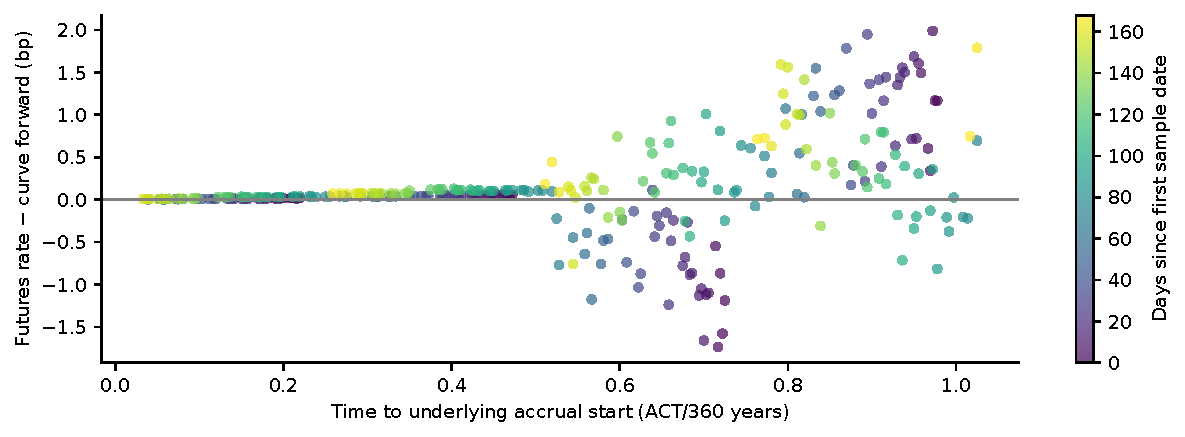
\includegraphics[width=.96\textwidth]{figures/empirical_convexity.pdf}
\caption{Observed SOFR futures rate minus the same-window forward rate from the Eris curve, in rate bp. Each point is a distinct date and underlying reference quarter. These are curve comparisons before any model convexity adjustment, execution costs, or intraday synchronization correction.}\label{fig:empiricalconvexity}
\end{figure}

Under the ideal Gaussian model, $p\geq0$, so a negative exact gap is incompatible with treating those inputs as a common exact model observation. It does not establish a tradable arbitrage in these datasets. Eris supplies a constructed curve, the observations are not synchronized executable quotes, and the traded swap's conventions may differ from \eqref{eq:oisforward}. The small median gap makes those distinctions consequential. A candidate trade would require an independently quoted, convention-matched OIS and an offsetting futures strip, with the residual outside the full adjustment and cost range. CME Clearing Advisory 23-050 specifies one monthly SOFR future and up to thirteen quarterly SOFR futures, alongside Eris swap futures and SOFR OIS, as inputs to the published Eris SOFR curve.\footnote{CME Clearing, 14 February 2023, effective 27 February 2023: \url{https://www.cmegroup.com/notices/clearing/2023/02/Chadv23-050.pdf}.} All 309 compared quarters start within 1.03 years, inside that maximum futures-input horizon. The public daily discount factors do not disclose the constituent set, fitting weights, or curve sensitivities, so an SR3 percentage contribution cannot be recovered from them. The documented input overlap is sufficient to rule out interpreting these small gaps as an independent market test of futures convexity.

